\documentclass{rapport}
\usepackage{lipsum}
\usepackage{gensymb}
\usepackage{float}
\usepackage{graphicx} % Required for inserting images
\usepackage{pythontex}
\usepackage{setspace}
\usepackage[skip=0pt]{caption}
\usepackage{booktabs}
\usepackage{tabularx}
\usepackage{amsmath}


\title{file title} %title of the file

\begin{document}
\onehalfspacing

%----------- Report information ---------

\logo{logos/DTU_Logo_Roed.jpg}
\uni{\textbf{Technical University of Denmark}}
\ttitle{Trading ETFs} %title of the file
\subject{Subject} % Subject name
\topic{Assignment 2} % Topic name

\students{\textsc{Visnukaran Kirubakaran, Student ID: s224527}} % information related to the students

%----------- Init -------------------
        
\buildmargins % display margins
\buildcover % create the front cover of the document
\toc % creates the table of contents

%------------ Report body ----------------
\section{Descriptive analysis}
\addcontentsline{toc}{subsubsection}{\textbf{a)} Description of the data material}
\subsubsection*{\textbf{a)} Beskrivelse af data materialet}
\noindent
The dataset consists of weekly returns for 95 ETFs. It contains 96 columns, with the first column representing the date, and the remaining columns showing the weekly returns for each ETF.
In this project, the focus will be on 4 specific ETFs: AGG, VAW, IWN, and SPY. These are considered quantitative variables, as they represent numerical data that can be analyzed and computed.
For each ETF, there are a total of 454 observations, starting from May 5, 2006 and ending on May 8, 2015. However, it is noted that there are some missing values in the dataset. 
This is evident from the irregular intervals between certain dates, indicating that data for some weeks is missing.


\addcontentsline{toc}{subsubsection}{\textbf{b)} Density histogram of the weekly returns from the ETF AGG}
\subsubsection*{\textbf{b)} Density histogram of the weekly returns from the ETF AGG}
\noindent
Below can the density histogram of the weekly returns from the ETF AGG be seen with an overlayed normal curve. 
\begin{figure}[H]
    \centering
    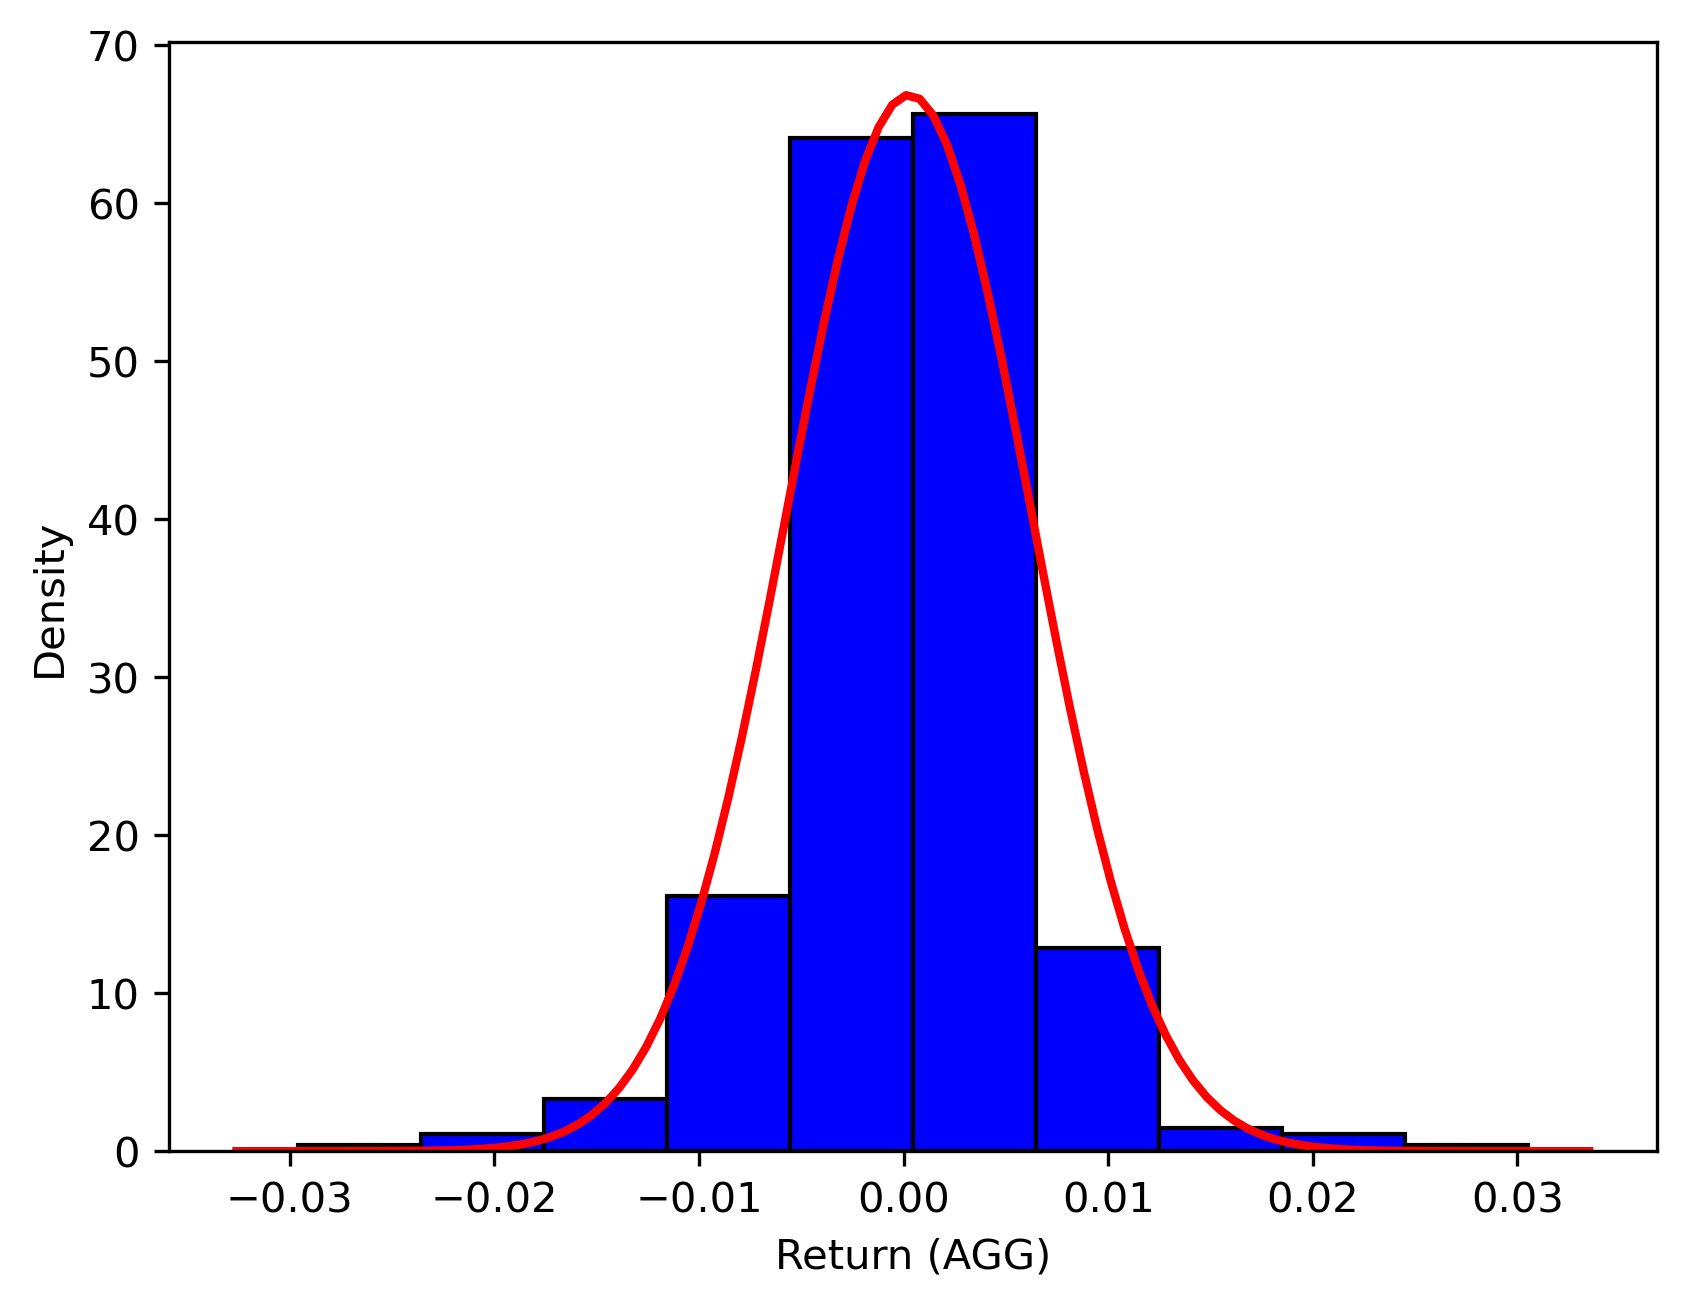
\includegraphics[width=0.75\textwidth]{histogram_with_normal_curve.png}  % Set width to 75% of text width
    \caption{\small Density histogram of the weekly returns from ETF AGG with normal distribution overlay.}  % Use smaller font for the caption
    \label{fig:histogram_AGG}
\end{figure}
\noindent
\noindent
%Use this histogram to describe the empirical distribution of the returns. Is the empirical
%density symmetrical or skewed? Can the returns be both positive and negative?
%Is there much variation to be seen in the observations?
The histogram can be seen as symmetrical because the mean and median of the ETF returns are close, indicating a balanced distribution of values around the center. 
This lack of skewness, combined with the equal spread of data on both sides of the mean, suggests the returns follow a roughly normal distribution.
Furtheremore, the return can both be seen in the positive and negative directions of the x-axis, 
meaning the return can be both. Lastly, the histrogram moderate variation in the data, as the data points are spread around the mean with a roughly bell-shaped curve. 
The central peak indicates that most observations are clustered around the mean, while the tails show fewer extreme values.  


\addcontentsline{toc}{subsubsection}{\textbf{c)} The weekly return over time for each of the four ETFs}
\subsubsection*{\textbf{c)} The weekly return over time for each of the four ETFs}
The four plots illustrate the weekly returns of different ETFs (AGG, VAW, IWN, and SPY) over time, showing distinct volatility patterns for each. 
AGG, being a bond ETF, has much smaller fluctuations in returns, reflecting its lower risk profile compared to the others. 
In contrast, VAW and IWN display larger and more frequent swings, indicating higher potential for both gains and losses. 
A common feature across all ETFs is the period of significant volatility between 2008 and 2009, likely due to the global financial crisis. 
Some instability is also observed around 2011, reflecting continued market uncertainty. 
These fluctuations suggest varying levels of market sensitivity, with AGG being more stable and VAW/IWN showing greater exposure to risk.

% Figur 2: AGG
\begin{figure}[H]
    \centering
    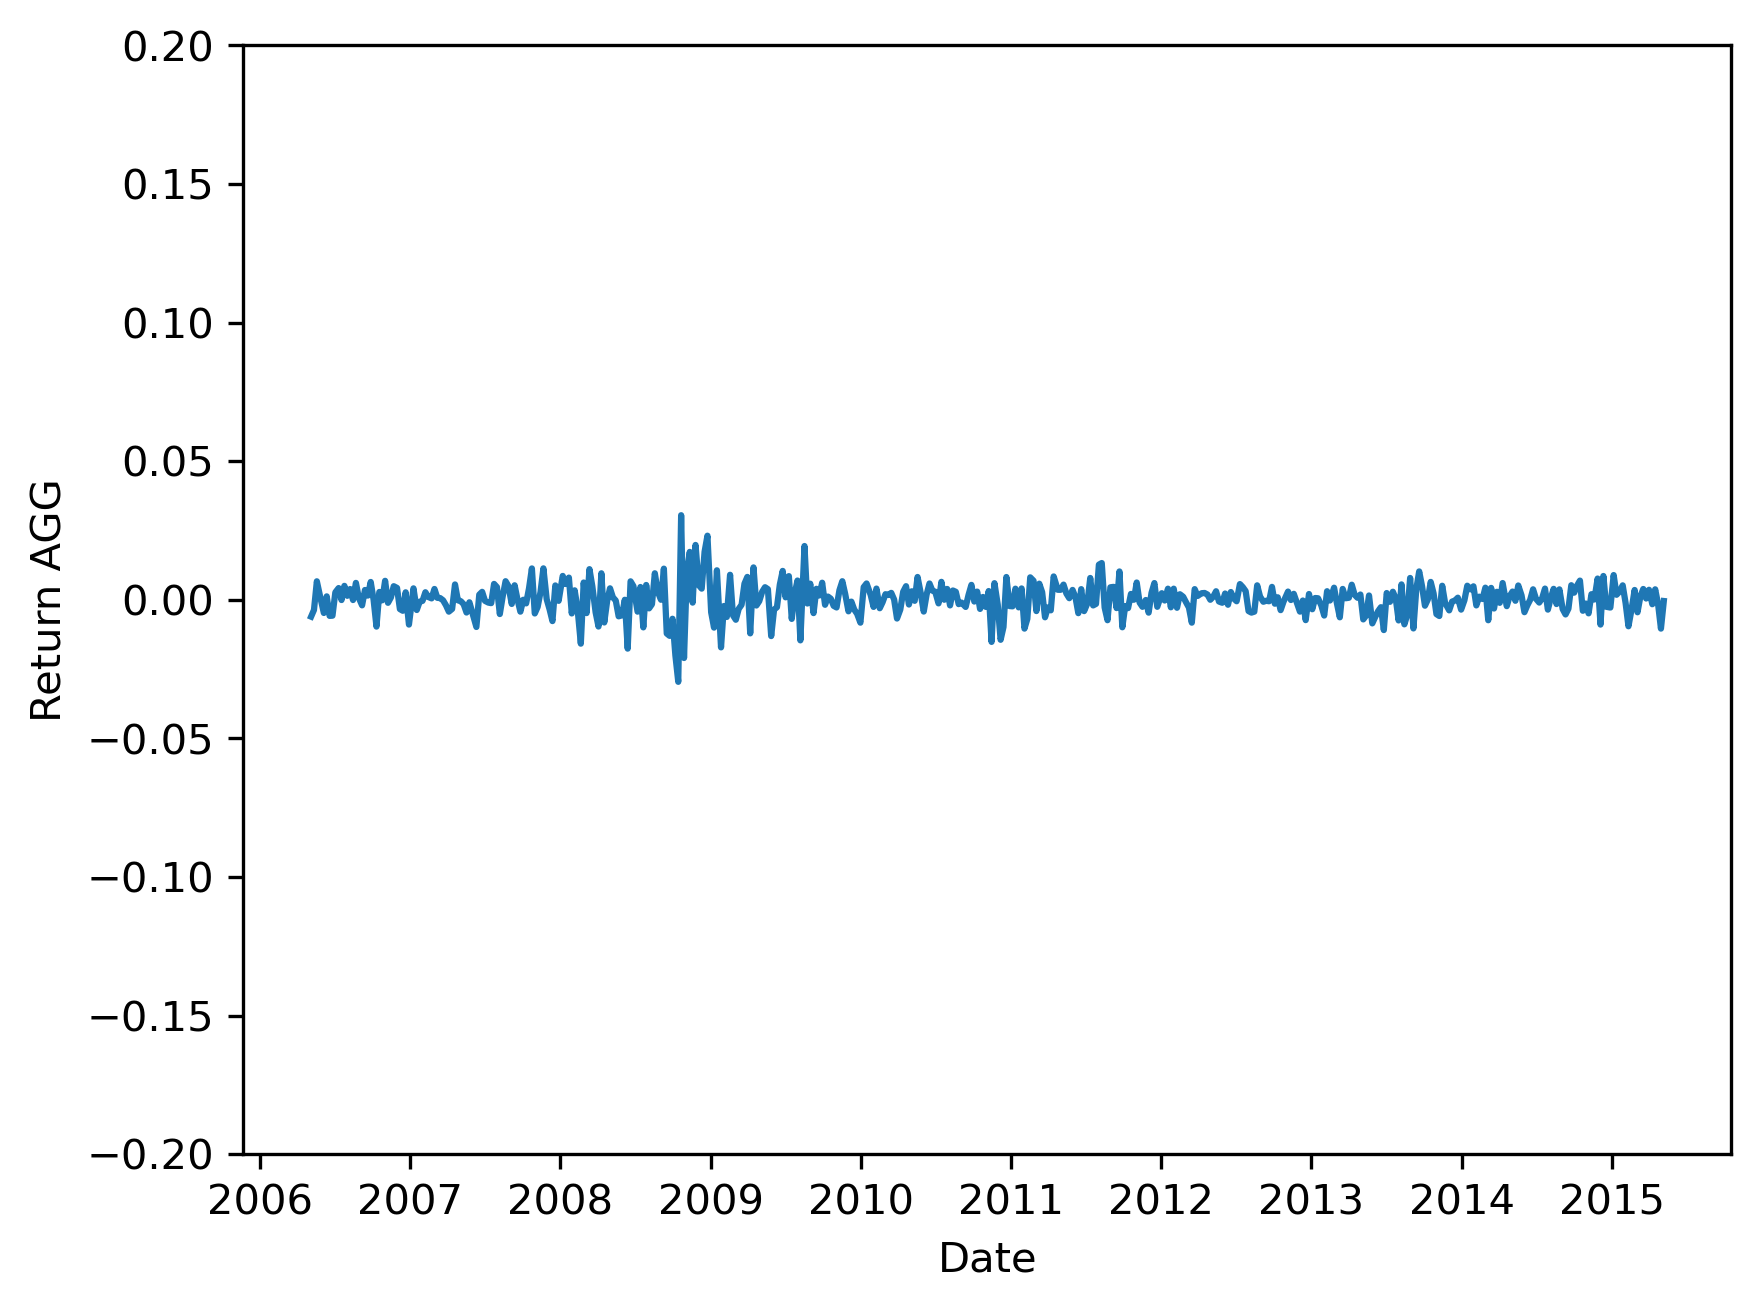
\includegraphics[width=0.7\textwidth]{figure_2_AGG_development.png}
    \caption{Figur 2: AGG's development over time}
    \label{fig:agg_development}
\end{figure}

% Figur 3: VAW
\begin{figure}[H]
    \centering
    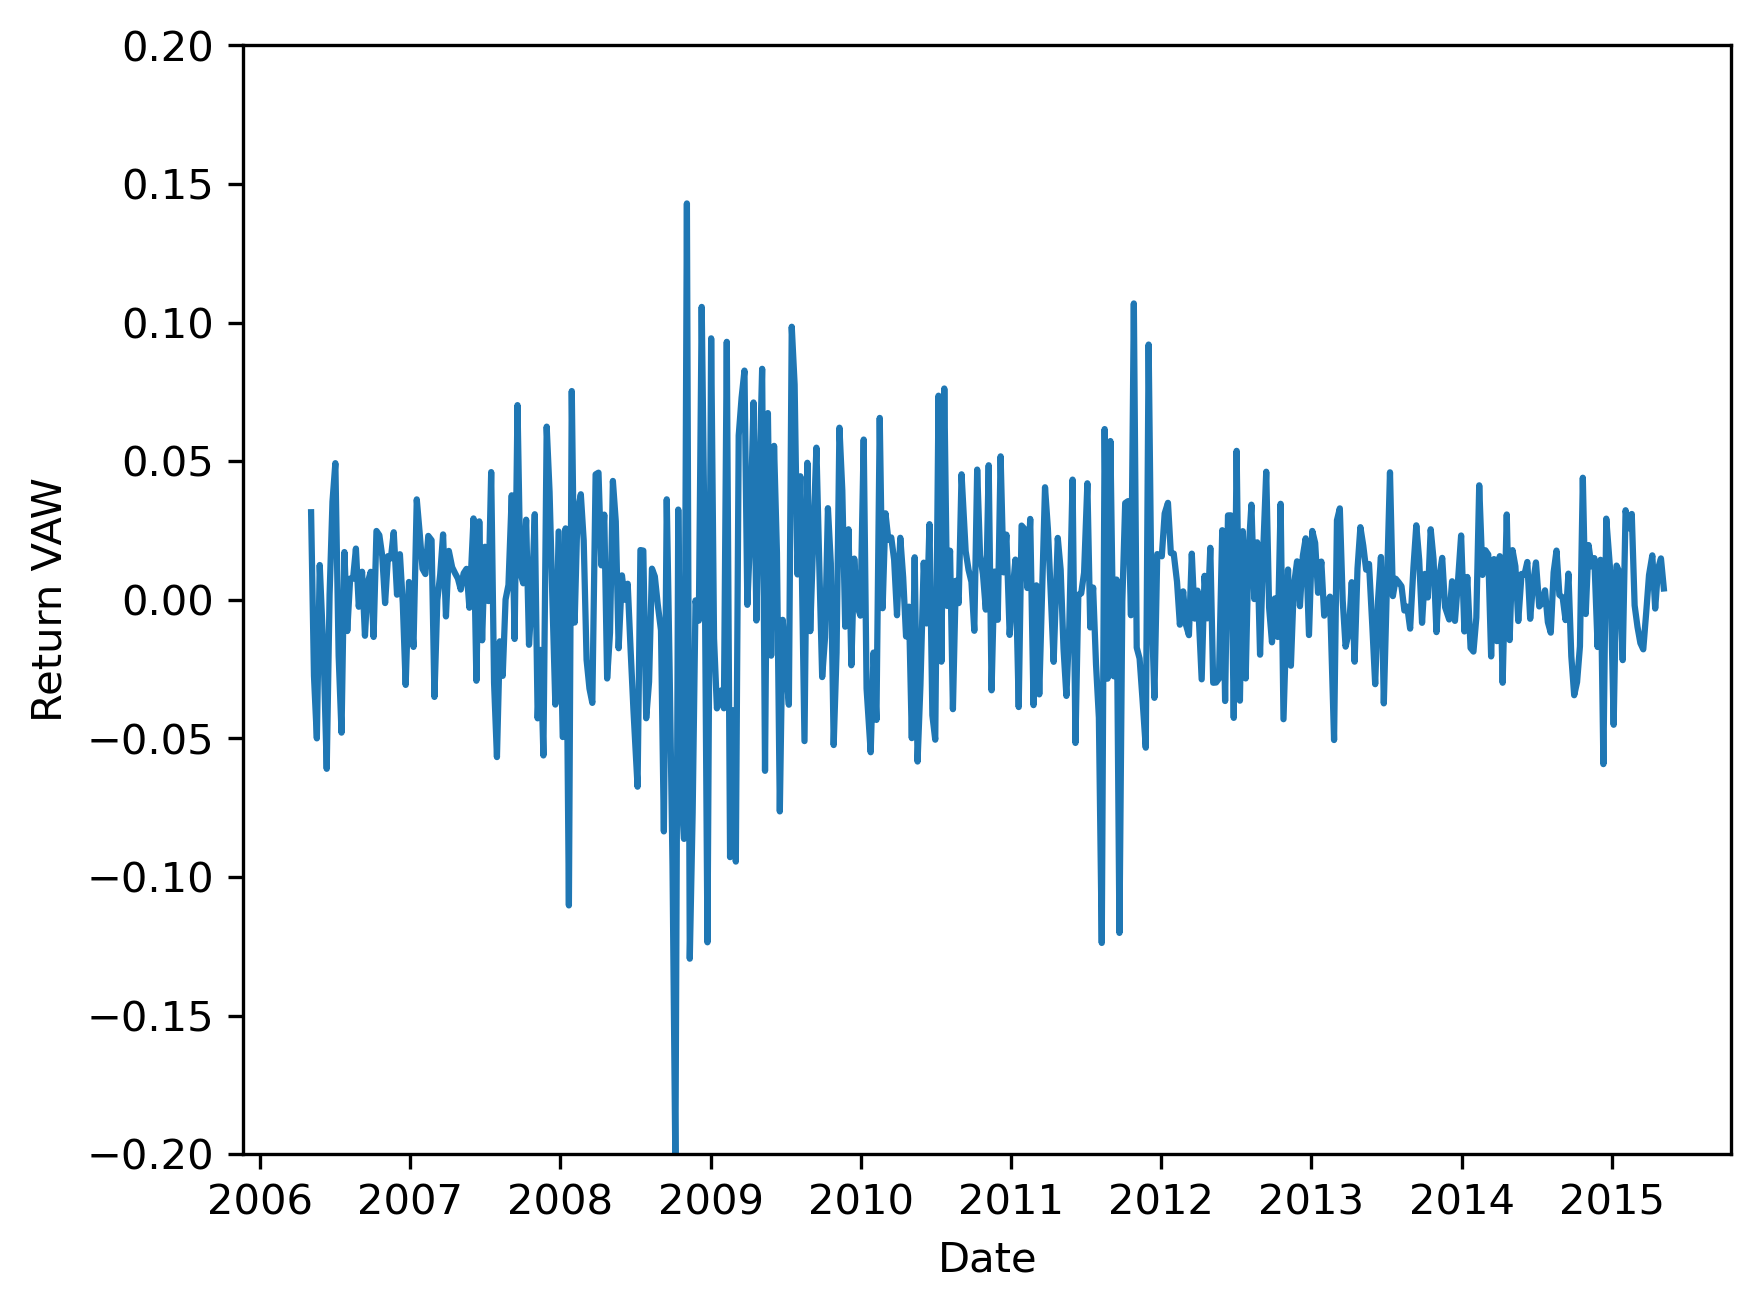
\includegraphics[width=0.7\textwidth]{figure_VAW_development.png}
    \caption{Figur 3: VAW's development over time}
    \label{fig:vaw_development}
\end{figure}

% Figur 4: IWN
\begin{figure}[H]
    \centering
    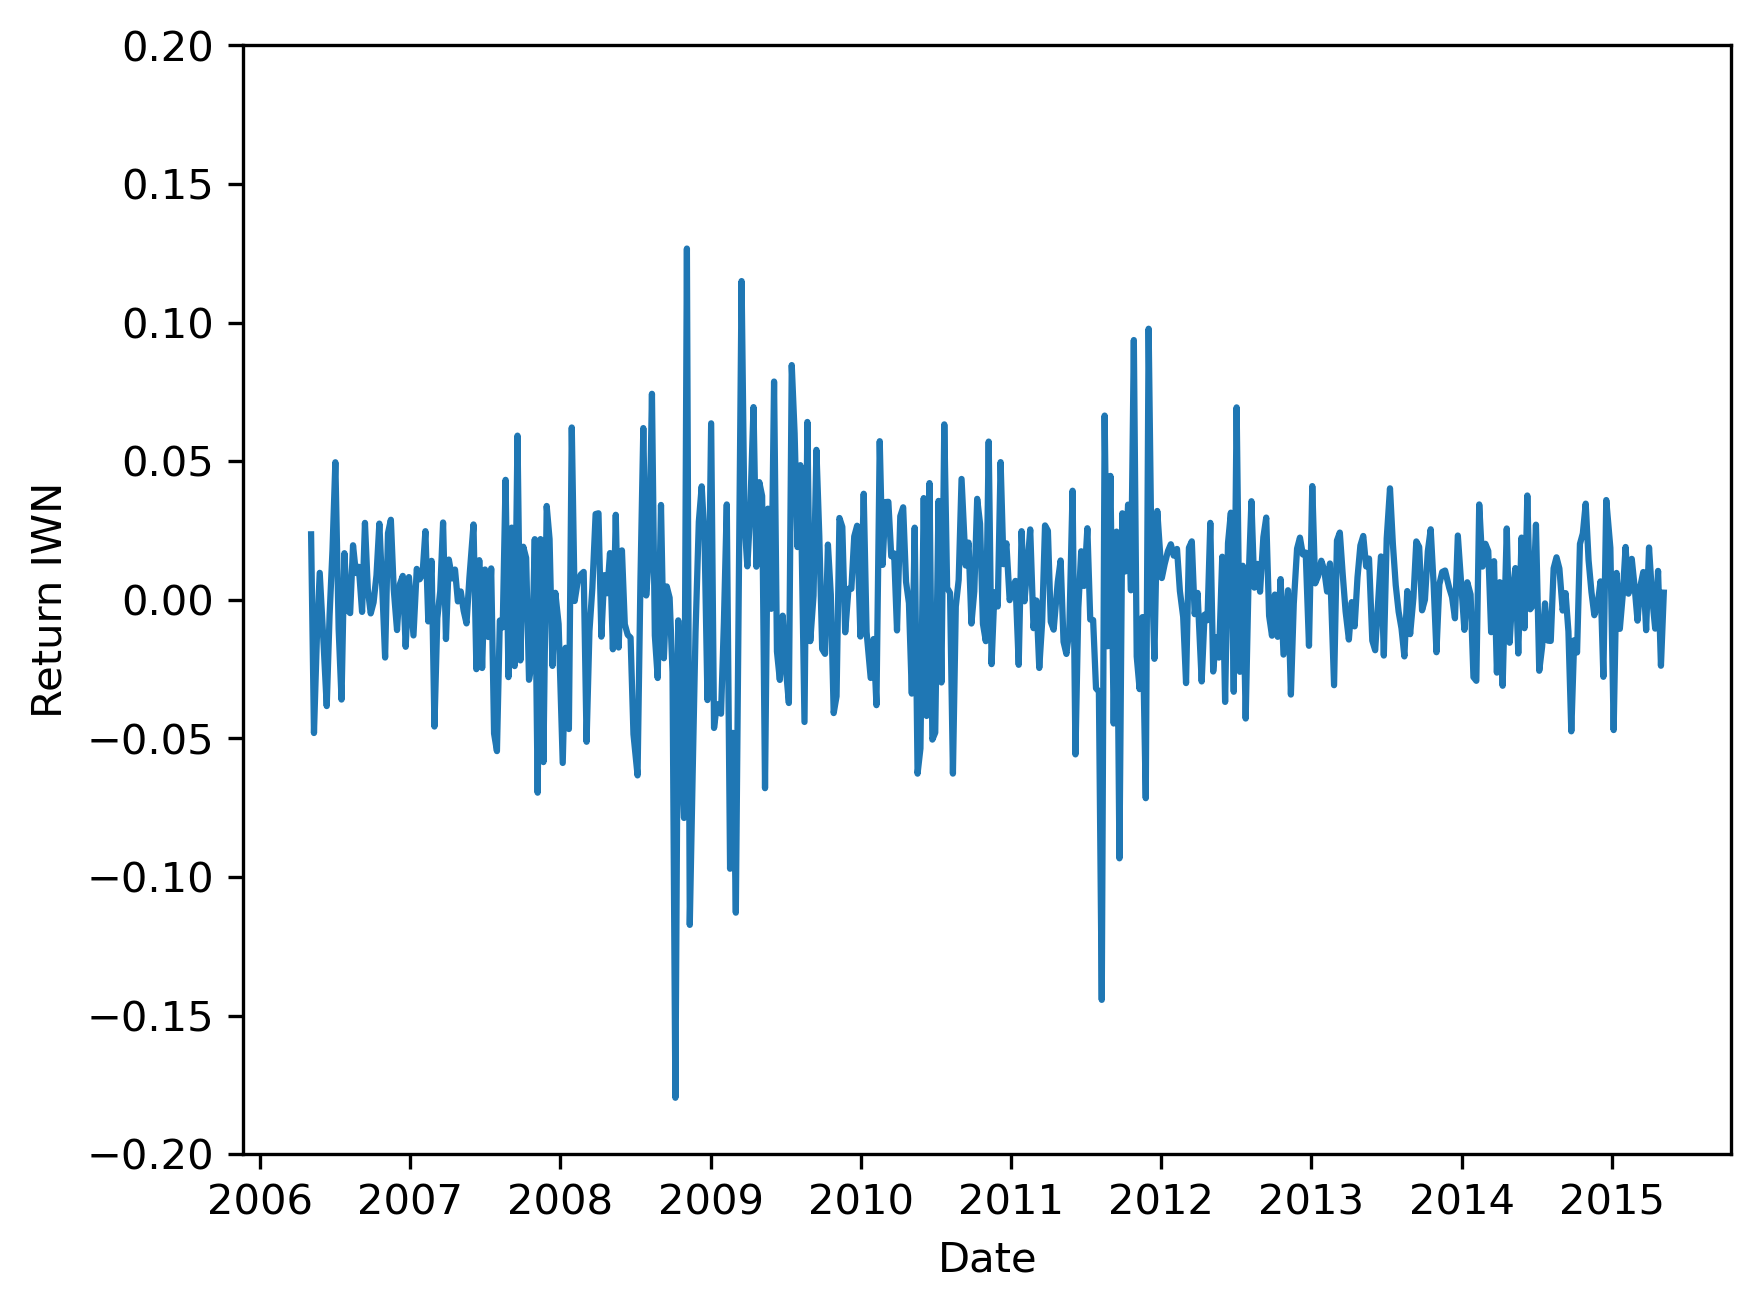
\includegraphics[width=0.7\textwidth]{figure_IWN_development.png}
    \caption{Figur 4: IWN's development over time}
    \label{fig:iwn_development}
\end{figure}

% Figur 5: SPY
\begin{figure}[H]
    \centering
    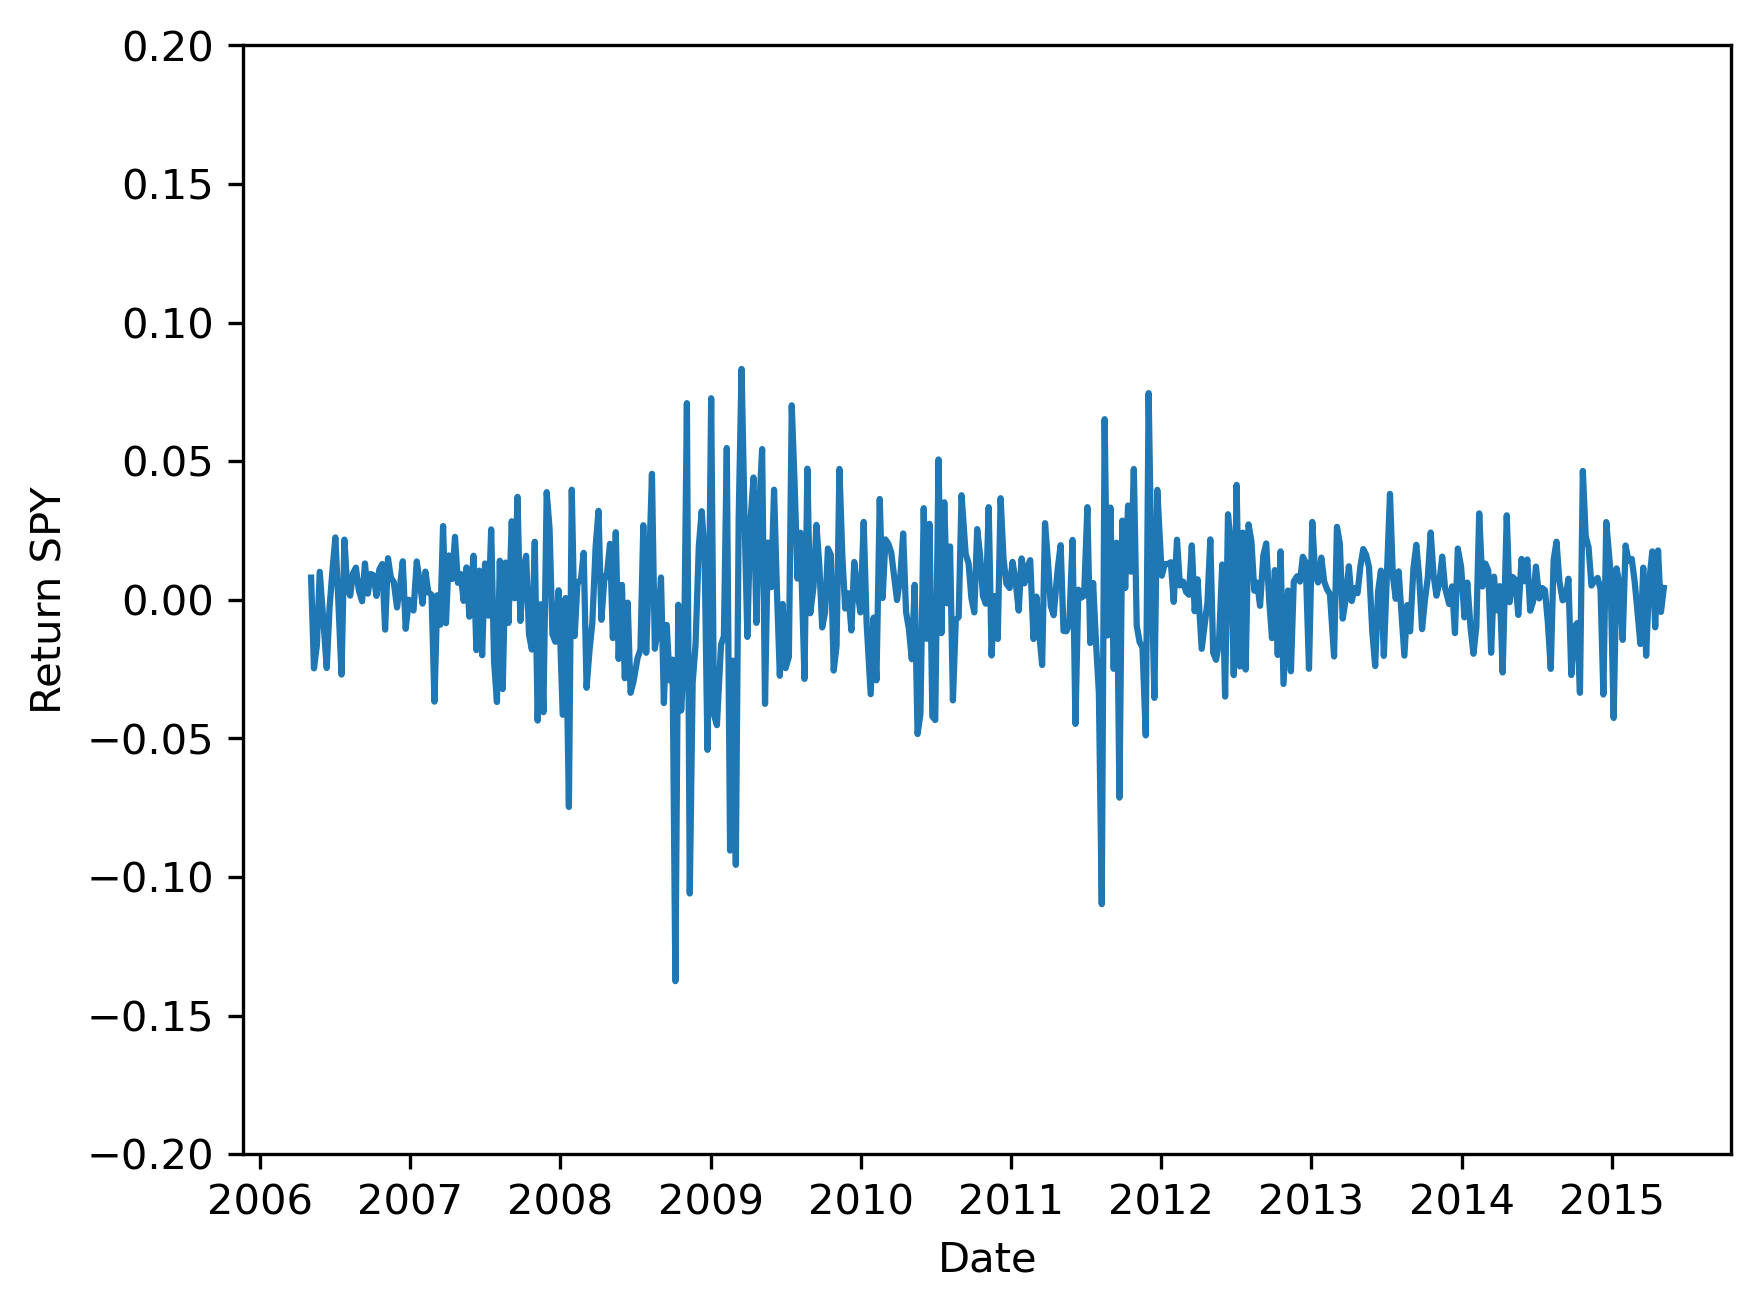
\includegraphics[width=0.7\textwidth]{figure_SPY_development.png}
    \caption{Figur 5: SPY's development over time}
    \label{fig:spy_development}
\end{figure}

\addcontentsline{toc}{subsubsection}{\textbf{d)} Box plot of the weekly returns by ETF}
\subsubsection*{\textbf{d)} Box plot of the weekly returns by ETF}
The box plot illustartes the empirical distribution of the weekly returns from each of the four ETFs
\begin{figure}[H]
    \centering
    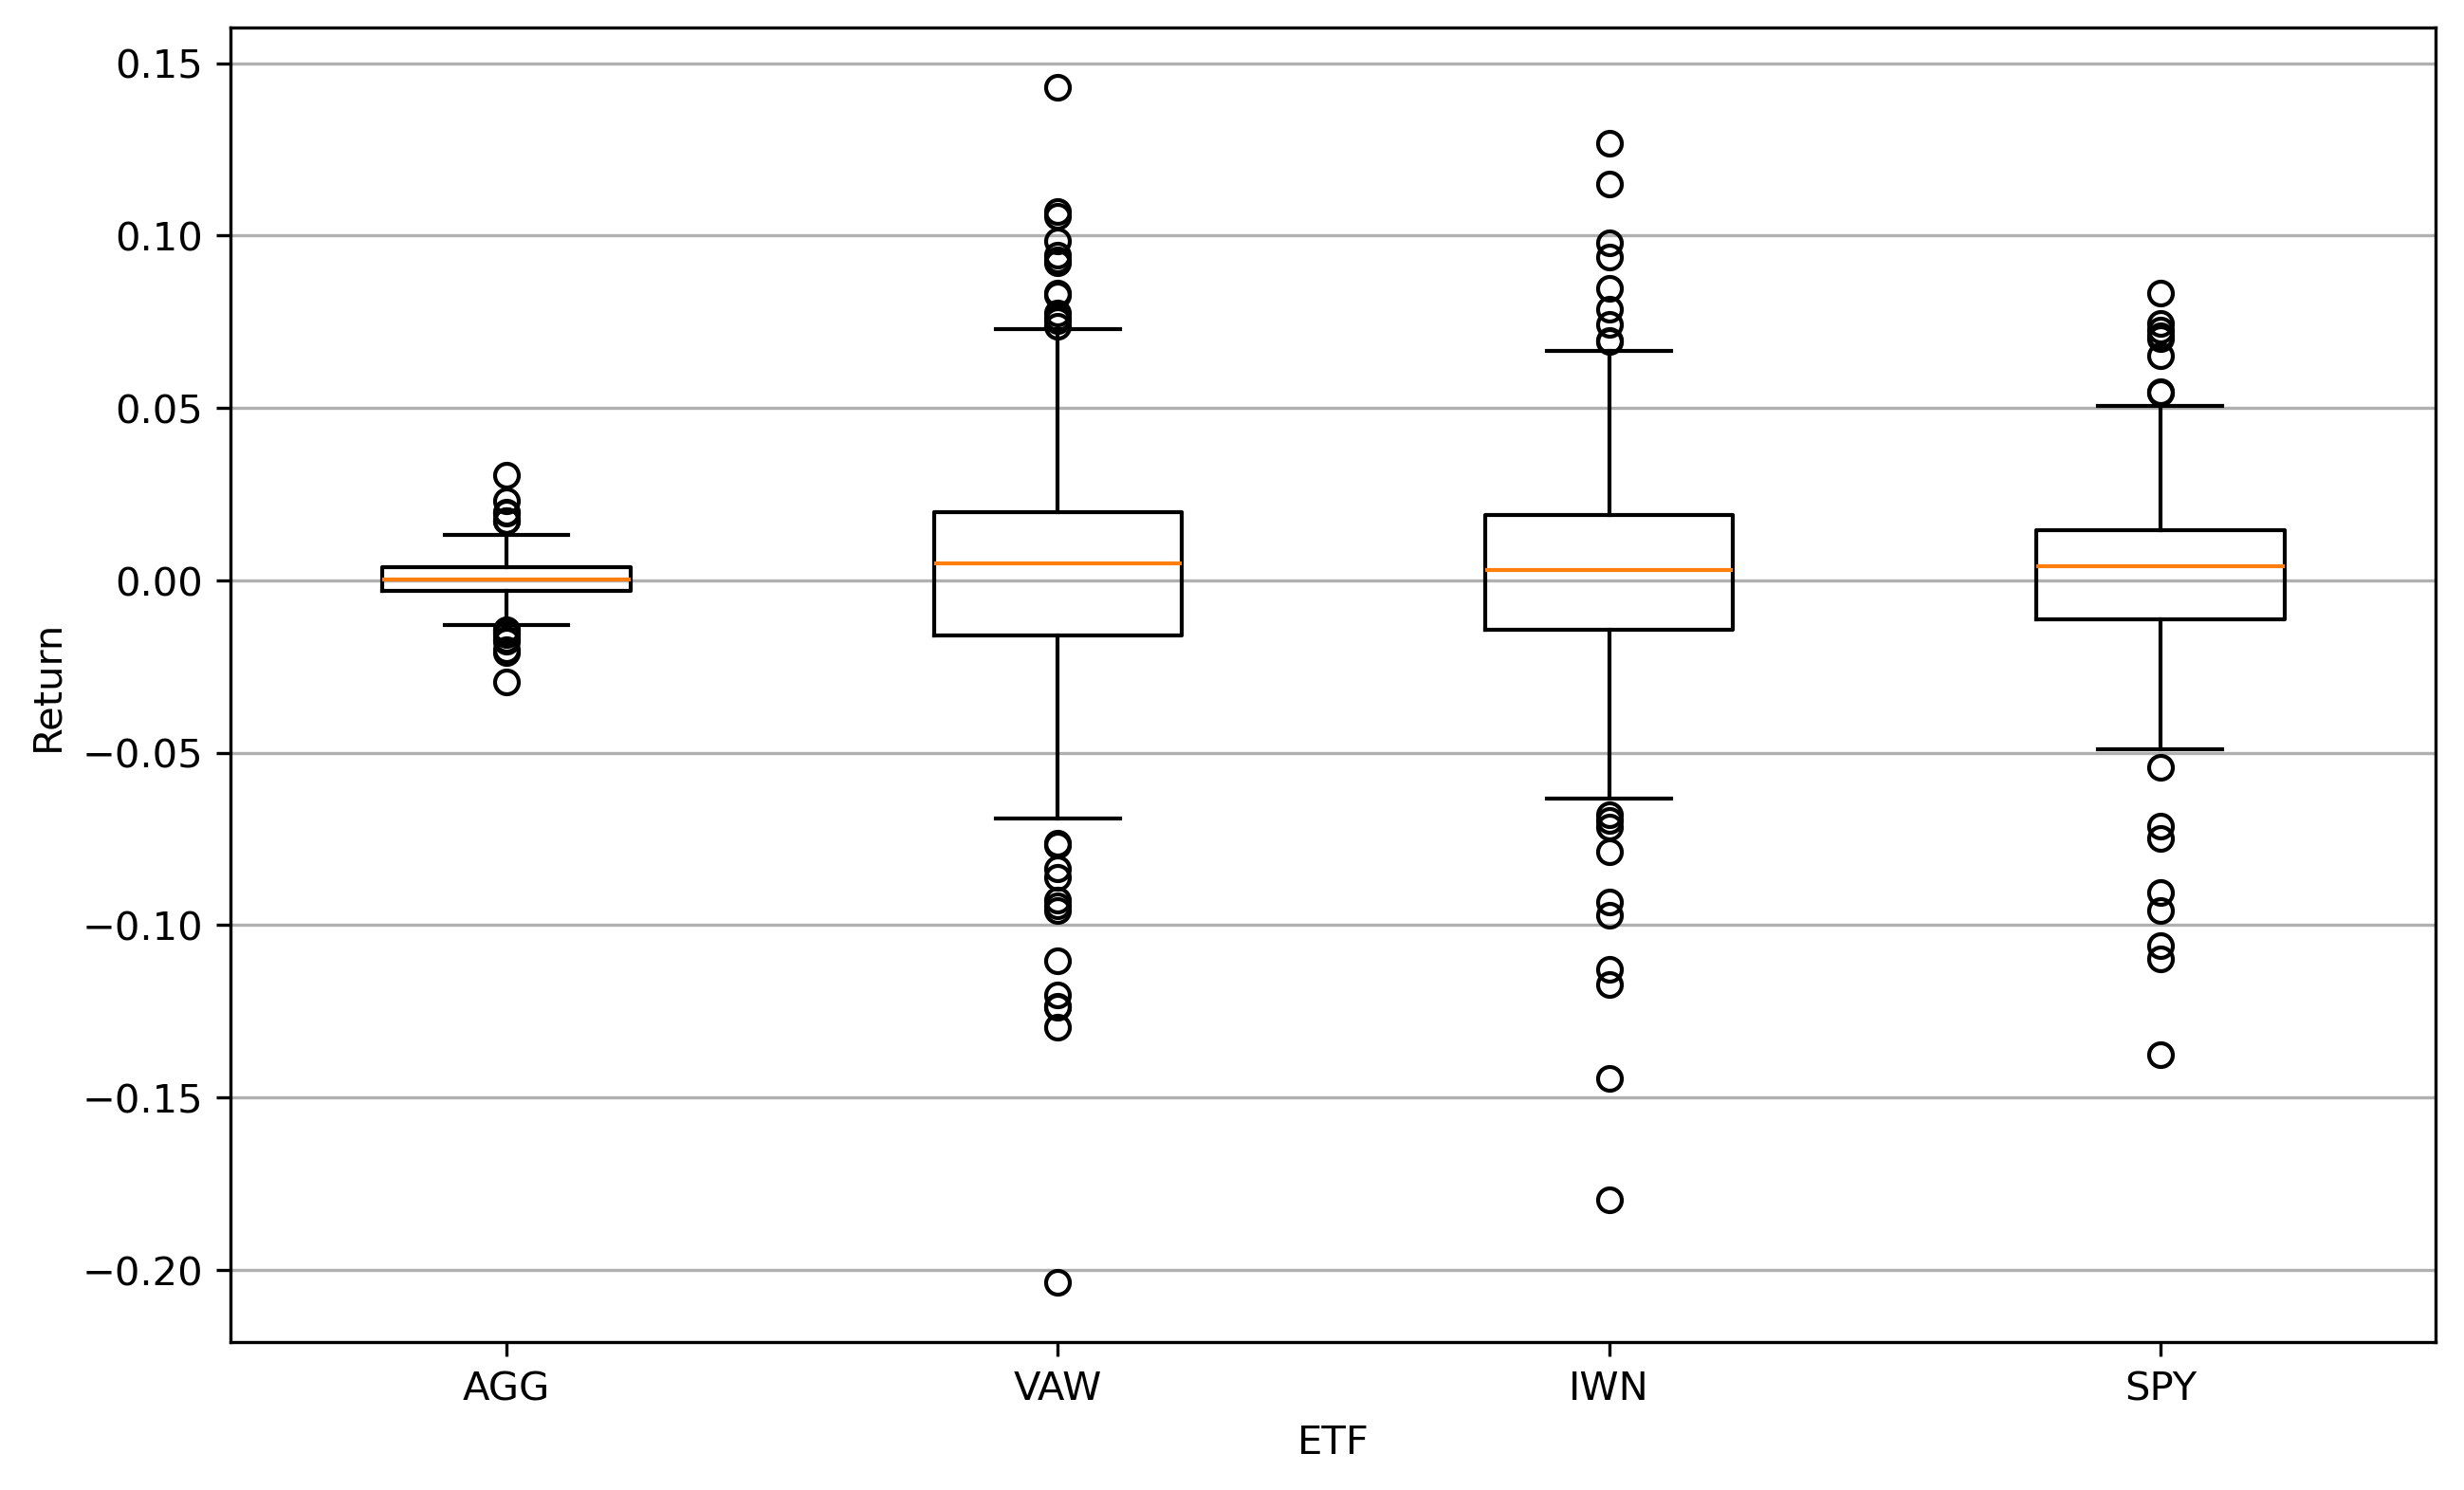
\includegraphics[width=0.75\textwidth]{figure_6_boxplot_of_returns.png}  % Set width to 75% of text width
    \caption{\small Boxplot of the weekly returns by ETF.}  % Use smaller font for the caption
    \label{fig:histogram_AGG}
\end{figure}
\noindent
\noindent
The box plot shows the distribution of weekly returns for the four ETFs (AGG, VAW, IWN, and SPY). 
AGG has the most compact and nearly symmetrical distribution, while VAW and SPY are left-skewed, with more negative returns. 
IWN is the most balanced, with returns spread symmetrically around the median. 
VAW has the largest variability, shown by its wide interquartile range (IQR), while AGG has the smallest. 
All ETFs display several outliers, particularly VAW and IWN, which could be due to market events during the period.

\addcontentsline{toc}{subsubsection}{\textbf{e)} Summary sizes for the four ETFs}
\subsubsection*{\textbf{e)} Summary sizes for the four ETFs}

\begin{table}[H]  % Create a table environment
    \centering  % Center the table
    \begin{tabularx}{\textwidth}{lXXXXXXX}
    \toprule
         & Number of obs. & Sample mean & Sample variance & Std. dev. & Lower quartile (Q1) & Median (Q2) & Upper quartile (Q3) \\
    \midrule
        AGG & 454.000000 & 0.000266 & 0.000036 & 0.005976 & -0.002973 & 0.000237 & 0.003893 \\
        VAW & 454.000000 & 0.001794 & 0.001302 & 0.036083 & -0.016096 & 0.004798 & 0.019685 \\
        IWN & 454.000000 & 0.001188 & 0.001025 & 0.032015 & -0.014305 & 0.003120 & 0.019056 \\
        SPY & 454.000000 & 0.001360 & 0.000614 & 0.024786 & -0.011325 & 0.004216 & 0.014498 \\
    \bottomrule
    \end{tabularx}
    \caption{Summary sizes for the four ETFs}  % Add the table caption below the table
\end{table}




The table provides precise values for the mean, variance, and standard deviation, which are not visible in the box plot. 
It also shows the exact number of observations and quartiles, offering more detailed insights than the visual representation of the box plot.





\pagebreak
\section{Statistical analysis}
\addcontentsline{toc}{subsubsection}{\textbf{f)} Statistical models describing the weekly return for each of the
four ETFs}
\subsubsection*{\textbf{f)} Statistical models describing the weekly return for each of the
four ETFs}

%pecify separate statistical models describing the weekly return for each of the
%four ETFs (see Remark 3.2)
The weekly returns from the four ETF's can be seperated into the following statistical models:

\begin{table}[H]
    \centering
    \begin{tabular}{|c|c|}
    \hline
    \textbf{ETF} & \textbf{Statistical Model} \\
    \hline
    AGG & $ AGG_i \sim \mathcal{N}(\mu_{AGG}, \sigma_{AGG}^2) $ and i.i.d., where $i = 1, ..., 454$ \\
    VAW & $ VAW_i \sim \mathcal{N}(\mu_{VAW}, \sigma_{VAW}^2) $ and i.i.d., where $i = 1, ..., 454$ \\
    IWN & $ IWN_i \sim \mathcal{N}(\mu_{IWN}, \sigma_{IWN}^2) $ and i.i.d., where $i = 1, ..., 454$ \\
    SPY & $ SPY_i \sim \mathcal{N}(\mu_{SPY}, \sigma_{SPY}^2) $ and i.i.d., where $i = 1, ..., 454$ \\
    \hline
    \end{tabular}
    \caption{Table 2: Statistical models for the weekly returns of the four ETFs}
\end{table}
\noindent
It is assumed that the observations in these statistical models are independent of each other, have the same distribution, and follow a normal distribution.

\noindent
The parameters for the models can furtheremore be estimated from the samle mean and the samle varians. 
These paaemeters where already found in section1, e, and can be seen here:
\begin{table}[H]  % Create a table environment
    \centering  % Center the table
    \begin{tabularx}{\textwidth}{lXXXXXXX}
    \toprule
         & Sample mean & Sample variance \\
    \midrule
        AGG & 0.000266 & 0.000036 \\
        VAW & 0.001794 & 0.001302 \\
        IWN & 0.001188 & 0.001025 \\
        SPY & 0.001360 & 0.000614 \\
    \bottomrule
    \end{tabularx}
    \caption{Estmated parameters}  % Add the table caption below the table
\end{table}



\pagebreak
\noindent
To perform model validation, QQ-plots for the four ETFs (AGG, VAW, IWN, and SPY) were compared with QQ-plots from simulated normal data.
\begin{figure}[H]
    \centering
    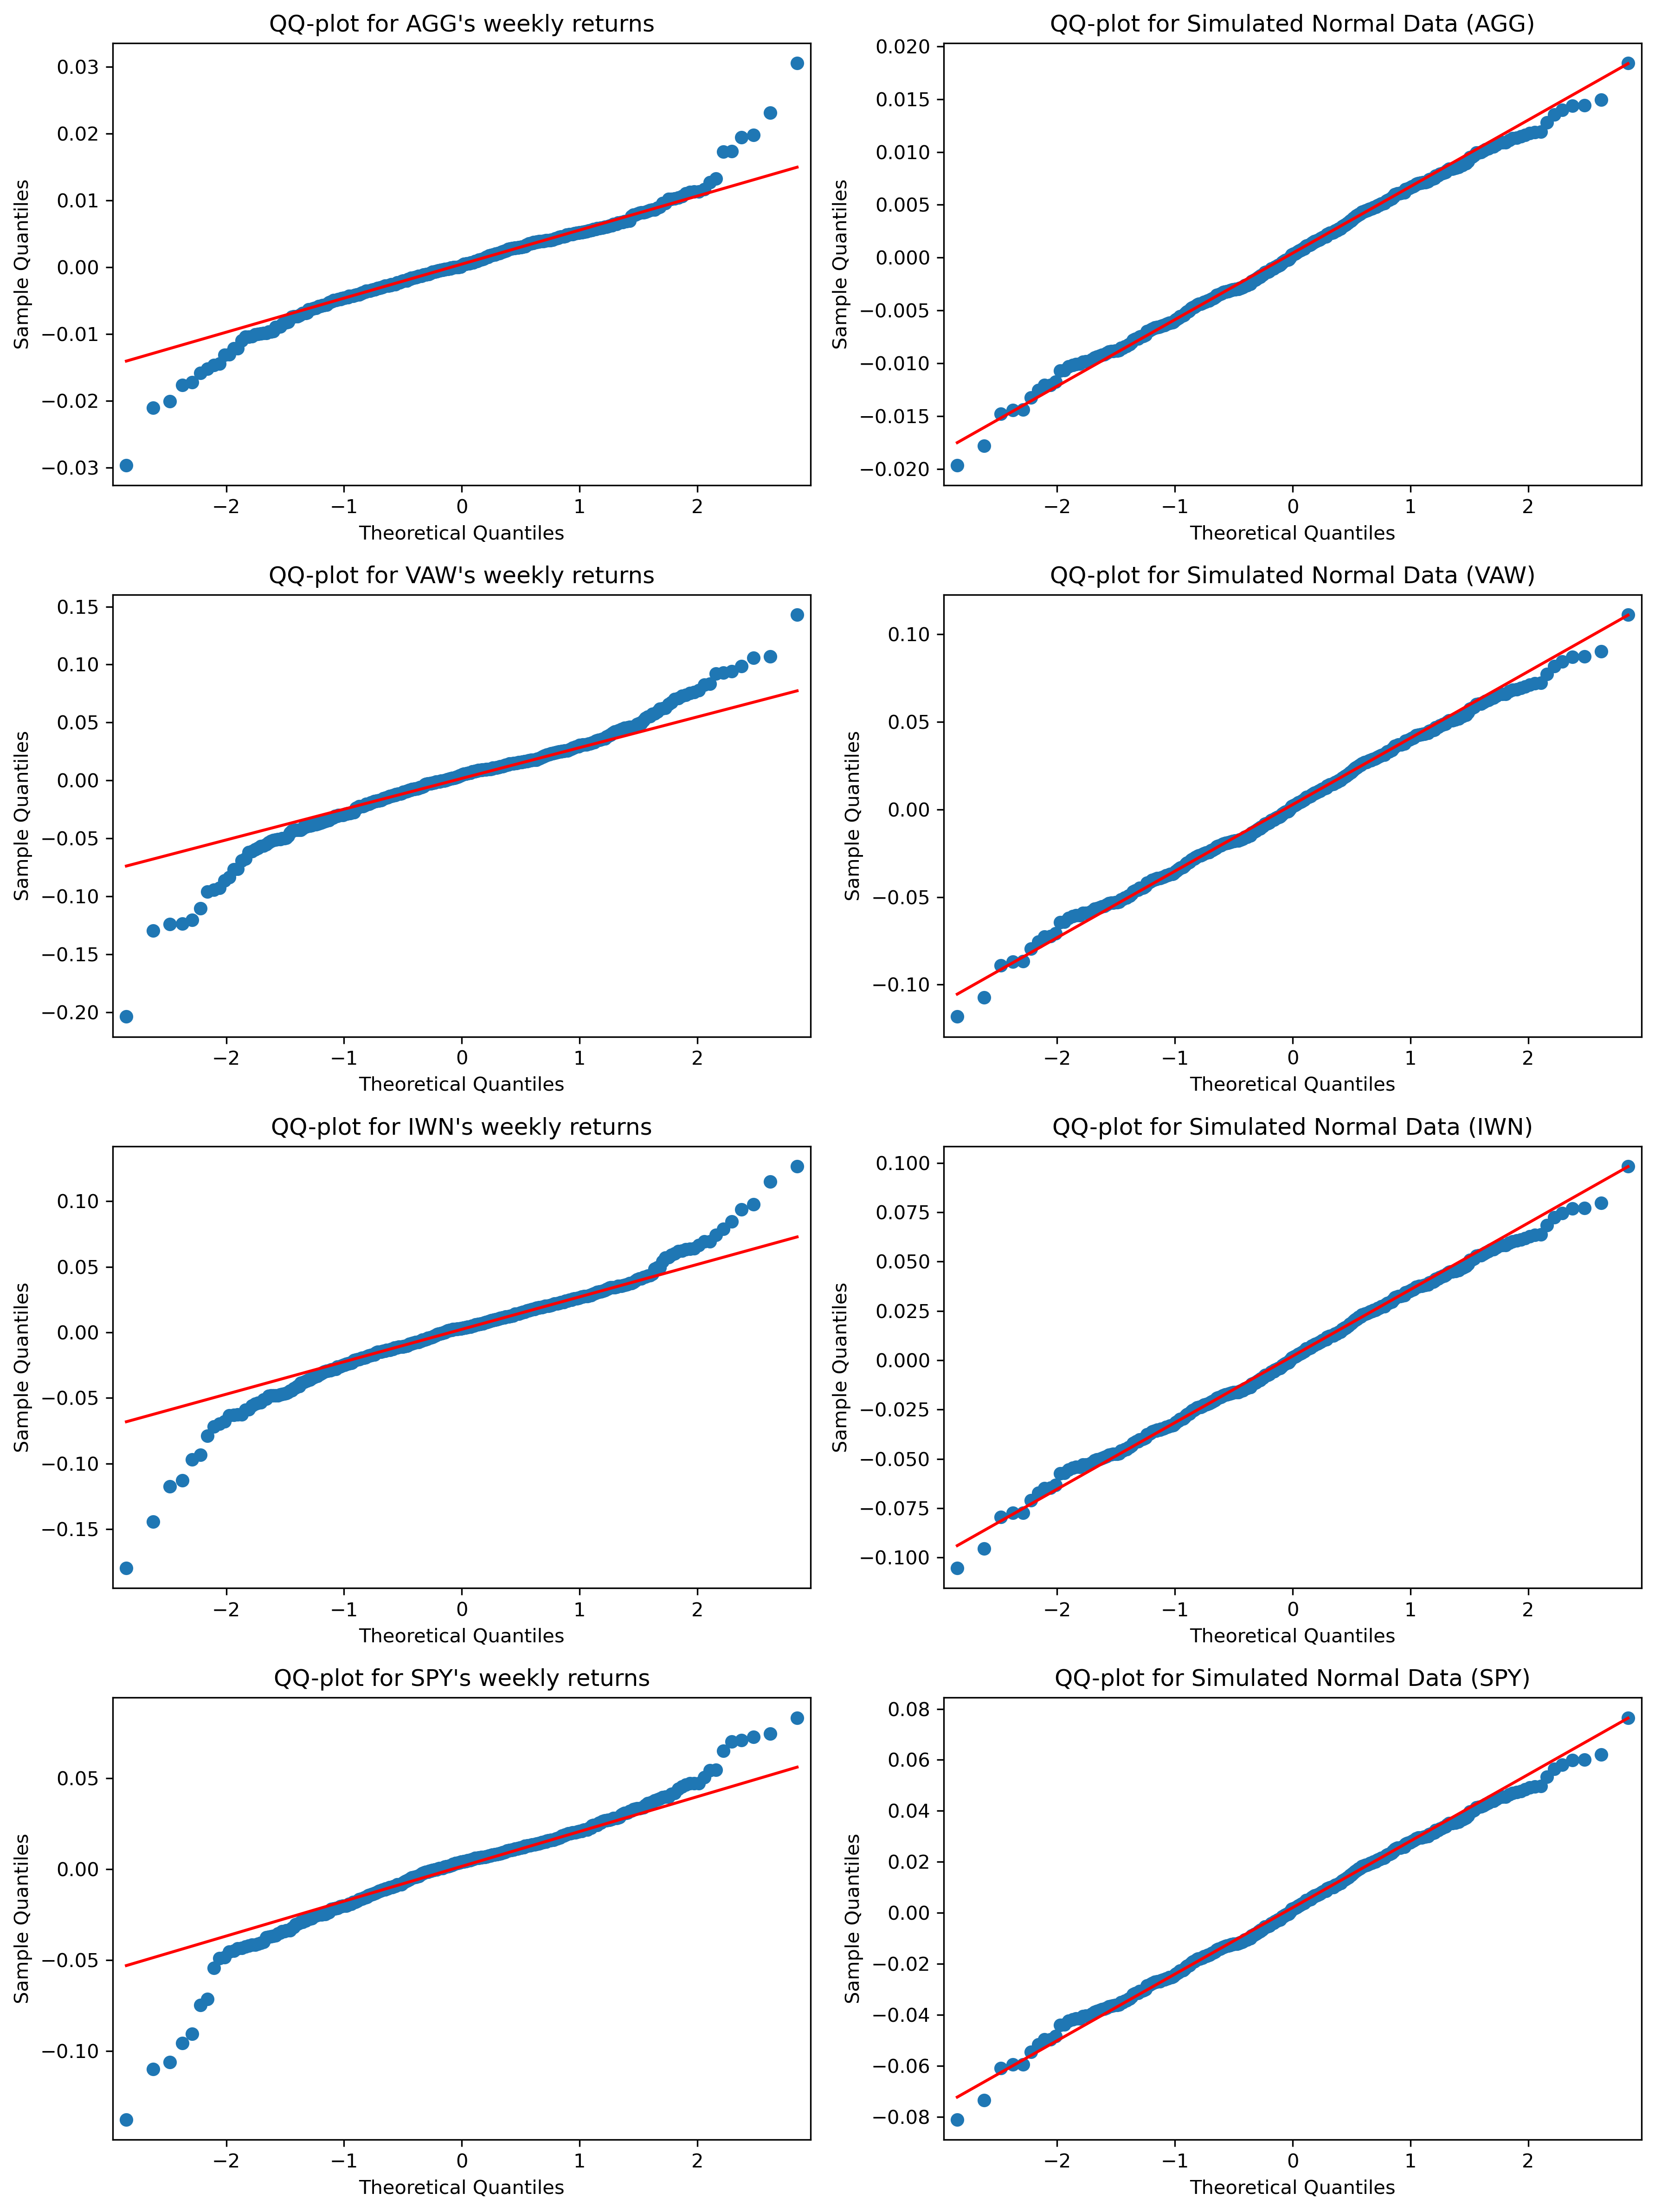
\includegraphics[width=0.85\textwidth]{figure_7_QQ_plots.png}  % Set width to 75% of text width
    \caption{\small QQ-plots of the ETF's and simulations.}  % Use smaller font for the caption
    \label{fig:histogram_AGG}
\end{figure}
\noindent
 
The observed ETF data deviates from normality, particularly in the tails, which suggests some degree of non-normality in the weekly returns. 
In contrast, the simulated data follows the expected normal distribution more closely.
However, due to the large sample size (454 observations for each ETF), the Central Limit Theorem (CLT) becomes important. 
The CLT states that the sample mean will approximate a normal distribution, even if the underlying data is not perfectly normal. 
Thus, the models are still reliable for further analysis, supported by the CLT, which can be expressed as:

\begin{equation}
    \frac{\overline{X} - \mu}{\sigma / \sqrt{n}} \sim N(0, 1^2)
    \label{eq:CLT}
    \end{equation}
    
\noindent


\addcontentsline{toc}{subsubsection}{\textbf{g)} Confidence intervals}
\subsubsection*{\textbf{g)} Confidence intervals}
\noindent
To calculate the 95\% confidence interval (CI) for the mean weekly return of AGG, we use the t-distribution with 
n-1 degrees of freedom, where n is the sample size (454 observations). 
The 0.975 quantile from the t-distribution is used to capture the central 95\% of the distribution.
The following equation can be used:

\[
\bar{x} \pm t_{1-\alpha/2} \cdot \frac{s}{\sqrt{n}}
\]
\noindent
We can find the critical t value using simple python where we get the value 1.9652145681681557. 
Now we can calculate the CI for the mean weekly return of AGG using the formular:
The mean we found in section f) to be 0.000265757 and the sample standard deviation from section e) to be 0.00597584. Now we can calculate it for AGG.
AGG: $\bar{x} \pm t_{1-\alpha/2} \cdot \frac{s}{\sqrt{n}} = 0.000265757 \pm 1.97 \cdot \frac{0.005976}{\sqrt{454}} = -0.0002867641 \ \text{og} \ 0.0008182781$.
\noindent
We can compute the corresponding intervals for the three remaining ETFs and fill it in a table:

\begin{table}[H]
    \centering
    \begin{tabular}{|l|c|c|}
    \hline
    \textbf{ETF} & \textbf{Lower bound of CI} & \textbf{Upper bound of CI} \\ \hline
    AGG  & -0.000285407345518444 & 0.0008169212976295796 \\ \hline
    VAW  & -0.0015342078012798403 & 0.005121788040169244 \\ \hline
    IWN  & -0.0017651741507074973 & 0.004140532646420902 \\ \hline
    SPY  & -0.0009259600489804174 & 0.0036461709486724178 \\ \hline
    \end{tabular}
    \caption{Confidence intervals for the four ETFs}
\end{table}
\noindent
When we compare the caculated CI for AGG with the given python code, it can be seen that the results are nearly equal with small rounding differences. 

\addcontentsline{toc}{subsubsection}{\textbf{h)} Hypothesis test}
\subsubsection*{\textbf{h)} Hypothesis test}

To test whether the mean weekly return for AGG deviates significantly from zero, we set up the following hypotheses:
\[
H_0: \mu_{AGG} = 0 \quad \text{and} \quad H_1: \mu_{AGG} \neq 0
\]
We perform the test at the 5\% significance level (\( \alpha = 0.05 \)) and calculate the t-statistic using the formula:
\[
t = \frac{\bar{x} - \mu_0}{s / \sqrt{n}}
\]
\noindent
We can insert the values, and then get:
\[
t_{obs} = \frac{0.000265757 - 0}{\frac{0.005975841}{\sqrt{454}}} = 0.9475750245
\]

\noindent
The p value can be calculated as follows:

\[
p\text{-value} = 2 \cdot P(T > |t_{obs}|) = 2 \cdot P(1.97 > 0.948) = 0.3439
\]

\noindent
\textbf{Conclusion:} The hypothesis test suggests that the mean weekly return for AGG does not significantly deviate from zero. This conclusion aligns with the confidence interval calculated earlier, which also contained zero within its range, further supporting the result that the mean return is not statistically different from zero at the 95\% confidence level.

\noindent
Thus, performing the hypothesis test confirms the conclusion we obtained from the confidence interval, and we do not need to reject the model.
Furtheremore, the calculated results are equal to the results found in python. 


\addcontentsline{toc}{subsubsection}{\textbf{i)} Hypothesis Test: Comparison of Weekly Returns from VAW and AGG}
\subsubsection*{\textbf{i)} Hypothesis Test: Comparison of Weekly Returns from VAW and AGG}
\noindent
To investigate whether the mean weekly returns of VAW and AGG differ, we perform a Welch two-sample t-test. The hypothesis test is formulated as follows:


\begin{align*}
    H_0 &: \mu_{\text{VAW}} = \mu_{\text{AGG}} \\
    H_1 &: \mu_{\text{VAW}} \neq \mu_{\text{AGG}}
\end{align*}

\noindent
The null hypothesis $H_0$ states that the mean weekly returns of VAW and AGG are equal, while the alternative hypothesis $H_1$ states that the mean weekly returns differ.

\noindent
\textbf{Significance Level:} \\
We set the significance level at $\alpha = 0.05$.

\noindent
\textbf{Test Statistic:} \\
Using the Welch two-sample t-test, the test statistic is calculated as:

\[
t_{\text{obs}} = \frac{(\bar{x}_{\text{VAW}} - \bar{x}_{\text{AGG}}) - \delta_0}{\sqrt{\frac{s_{\text{VAW}}^2}{n_{\text{VAW}}} + \frac{s_{\text{AGG}}^2}{n_{\text{AGG}}}}}
\]

\noindent
where:
\begin{itemize}
    \item $\bar{x}_{\text{VAW}} = 0.001794$ and $\bar{x}_{\text{AGG}} = 0.000266$ are the sample means of VAW and AGG.
    \item $s_{\text{VAW}}^2 = 0.001302$ and $s_{\text{AGG}}^2 = 0.000036$ are the sample variances.
    \item $n_{\text{VAW}} = 454$ and $n_{\text{AGG}} = 454$ are the sample sizes for VAW and AGG.
\end{itemize}

\noindent
If we insert the values we get:
\[
t_{\text{obs}} = \frac{(0.000265757 - 0.00179379) - 0}{\sqrt{\frac{0.005975841^2}{454} + \frac{0.03608286^2}{454}}} = -0.890
\]

\noindent
The degrees of freedom for the Welch t-test are calculated using the following formula:
\[
\nu = \frac{\left( \frac{s_{\text{VAW}}^2}{n_{\text{VAW}}} + \frac{s_{\text{AGG}}^2}{n_{\text{AGG}}} \right)^2}{\frac{\left( \frac{s_{\text{VAW}}^2}{n_{\text{VAW}}} \right)^2}{n_{\text{VAW}} - 1} + \frac{\left( \frac{s_{\text{AGG}}^2}{n_{\text{AGG}}} \right)^2}{n_{\text{AGG}} - 1}}
\]

\noindent
We again insert the values and get:

\[
v = \frac{\left( \frac{0.005975841^2}{454} + \frac{0.03608286^2}{454} \right)^2}{\frac{\left( \frac{0.005975841^2}{454} \right)^2}{454-1} + \frac{\left( \frac{0.03608286^2}{454} \right)^2}{454-1}} = 478
\]

\noindent
The test statistic is computed as $0.890$:

\noindent
The corresponding p-value is $0.374$.

\noindent
Since the p-value of 0.374 is greater than the significance level of 0.05, we fail to reject the null hypothesis. This indicates that there is insufficient evidence to conclude that the mean weekly returns of VAW and AGG differ significantly.

\noindent
Thus, we conclude that the mean weekly returns of VAW and AGG are not significantly different, and there is no statistical evidence to suggest that one ETF has a higher mean return than the other.
Furtheremore, when we compare it to the python result, we get exact the same answer. 

\addcontentsline{toc}{subsubsection}{\textbf{j)} The importance of statistical test}
\subsubsection*{\textbf{j)} The importance of statistical test}
In task i, conducting the hypothesis test was essential because the confidence intervals from both ETFs overlapped. This overlap means the confidence intervals alone couldn't provide a clear conclusion about whether the mean returns differed. When confidence intervals overlap, additional testing is needed to draw any significant conclusions. Had there been no overlap, we could have dismissed the null hypothesis using just the confidence intervals. But since there was overlap, both the confidence intervals and the hypothesis test with a significance level of 
$\alpha$ = 5\% were required to arrive at a reliable result.


\addcontentsline{toc}{subsubsection}{\textbf{k)} Correlation between ETFs}
\subsubsection*{\textbf{k)} Correlation between ETFs}

\noindent
When constructing a portfolio of ETFs, the diversification of risk is crucial to reduce the overall volatility of the portfolio. 
One way to achieve diversification is by combining assets with low or negative correlations. 
The correlation between two ETFs measures how the returns of one ETF move relative to the other. 
In general, a negative or low correlation between two ETFs indicates a higher potential for diversification, as one ETF’s gain may offset the other’s loss, reducing the overall portfolio risk.

\noindent
The sample covariance between two ETFs is computed using the following formula:
\[
s_{xy} = \frac{1}{n-1} \sum_{i=1}^n (x_i - \bar{x})(y_i - \bar{y})
\]
where:
\begin{itemize}
    \item \( s_{xy} \) is the sample covariance,
    \item \( x_i \) and \( y_i \) are the individual returns for the two ETFs,
    \item \( \bar{x} \) and \( \bar{y} \) are the means of the returns for each ETF,
    \item \( n \) is the number of observations.
\end{itemize}

\noindent
The sample correlation coefficient is calculated as follows:
\[
r = \frac{s_{xy}}{s_x \cdot s_y}
\]
where:
\begin{itemize}
    \item \( s_x \) and \( s_y \) are the sample standard deviations of the two ETFs,
    \item \( s_{xy} \) is the sample covariance computed above.
\end{itemize}

\noindent
We can insert our values, and calculate the correlation:

\[
r = \frac{0.000984}{0.036083 \cdot 0.032015} = 0.852
\]

\noindent
This high positive correlation suggests that the weekly returns of VAW and IWN tend to move together in the same direction. This is consistent with the expectation, as both ETFs may be influenced by similar market factors.

\noindent
We can further illustrate this relationship by creating a scatter plot of the weekly returns of VAW against IWN.
\begin{figure}[H]
    \centering
    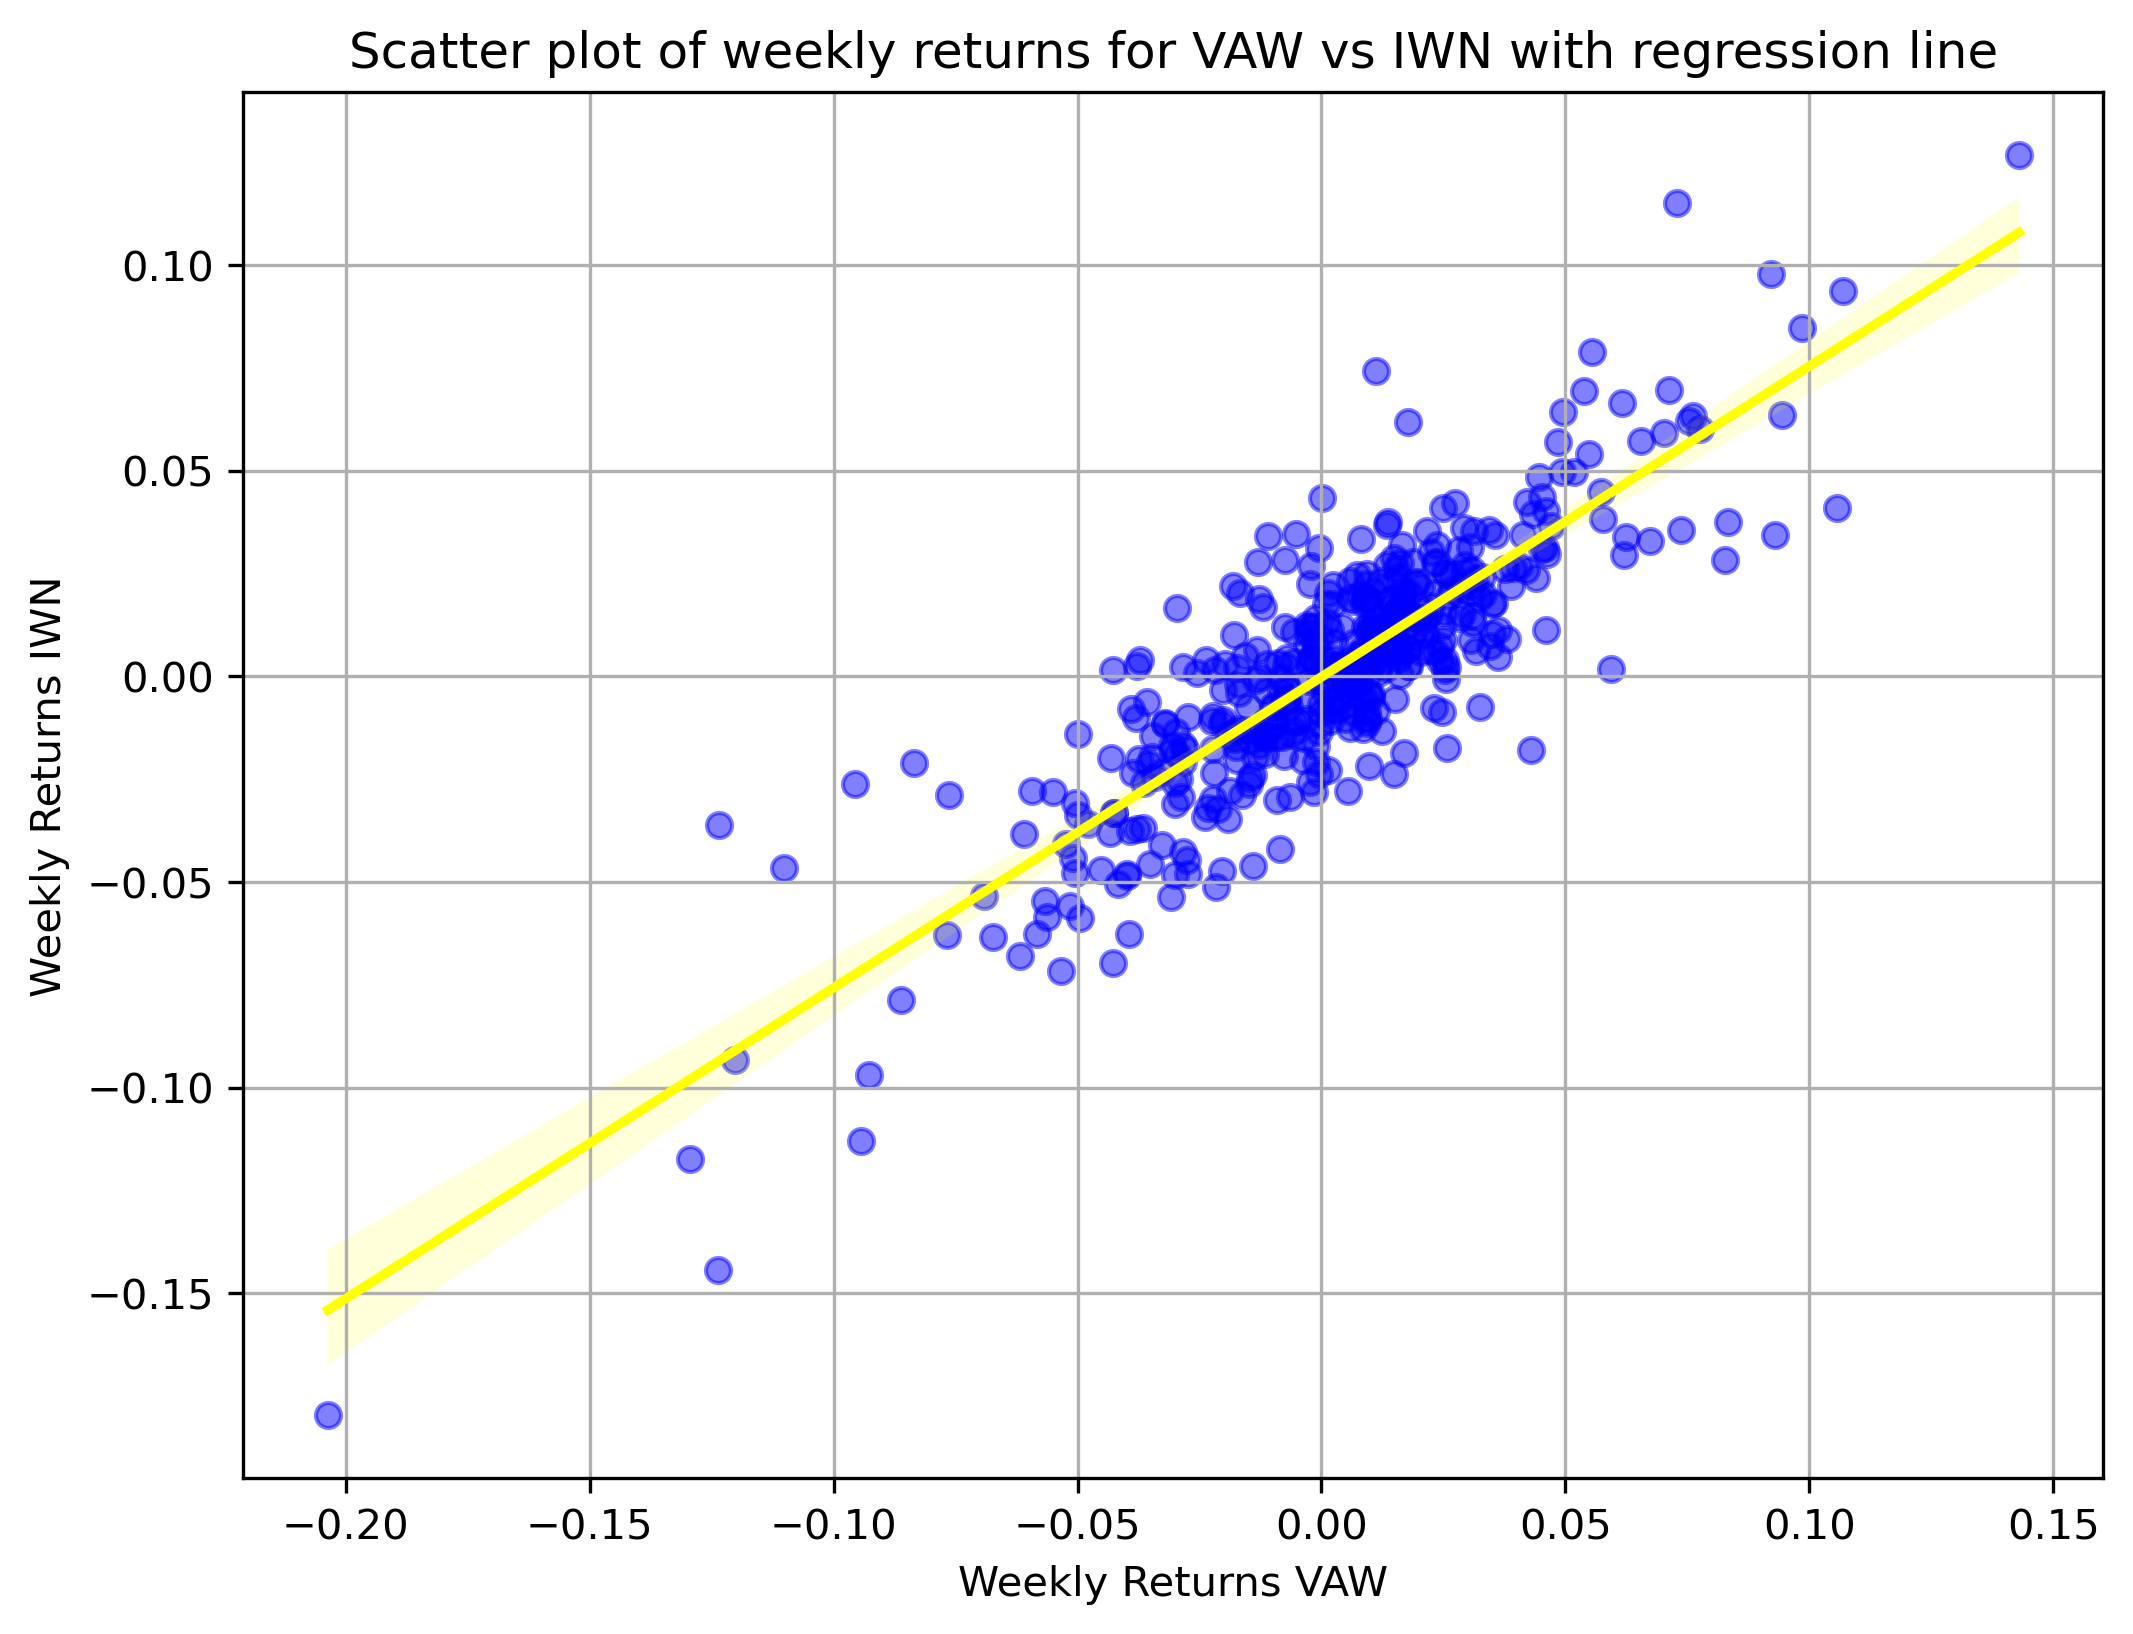
\includegraphics[width=0.75\textwidth]{figure_8_scatter_plot.png}  % Replace with the actual image file path
    \caption{\small Scatter plot of weekly returns for VAW vs. IWN.}
    \label{fig:scatter_vaw_iwn}
\end{figure}

\noindent
The scatter plot above demonstrates a positive linear relationship between the returns of VAW and IWN, which aligns with the high correlation coefficient observed. A strong positive correlation implies that the returns of both ETFs move similarly, indicating less opportunity for risk diversification by combining them in a portfolio.

\noindent
In conclusion, while combining VAW and IWN might still be part of a larger portfolio strategy, they would not provide substantial diversification benefits due to their high correlation.
\noindent
If we compare the correlation computed above to the python code, we get the exact same reult. 




\end{document}
